Na wykresie \ref{fig:CovValues} przedstawiono przykładowy przebieg wartości dla pierwszych 5 zmian
wraz z zaznaczonymi miejscami,
gdzie nastąpiła.
\begin{figure}[htbp]
  \centering
  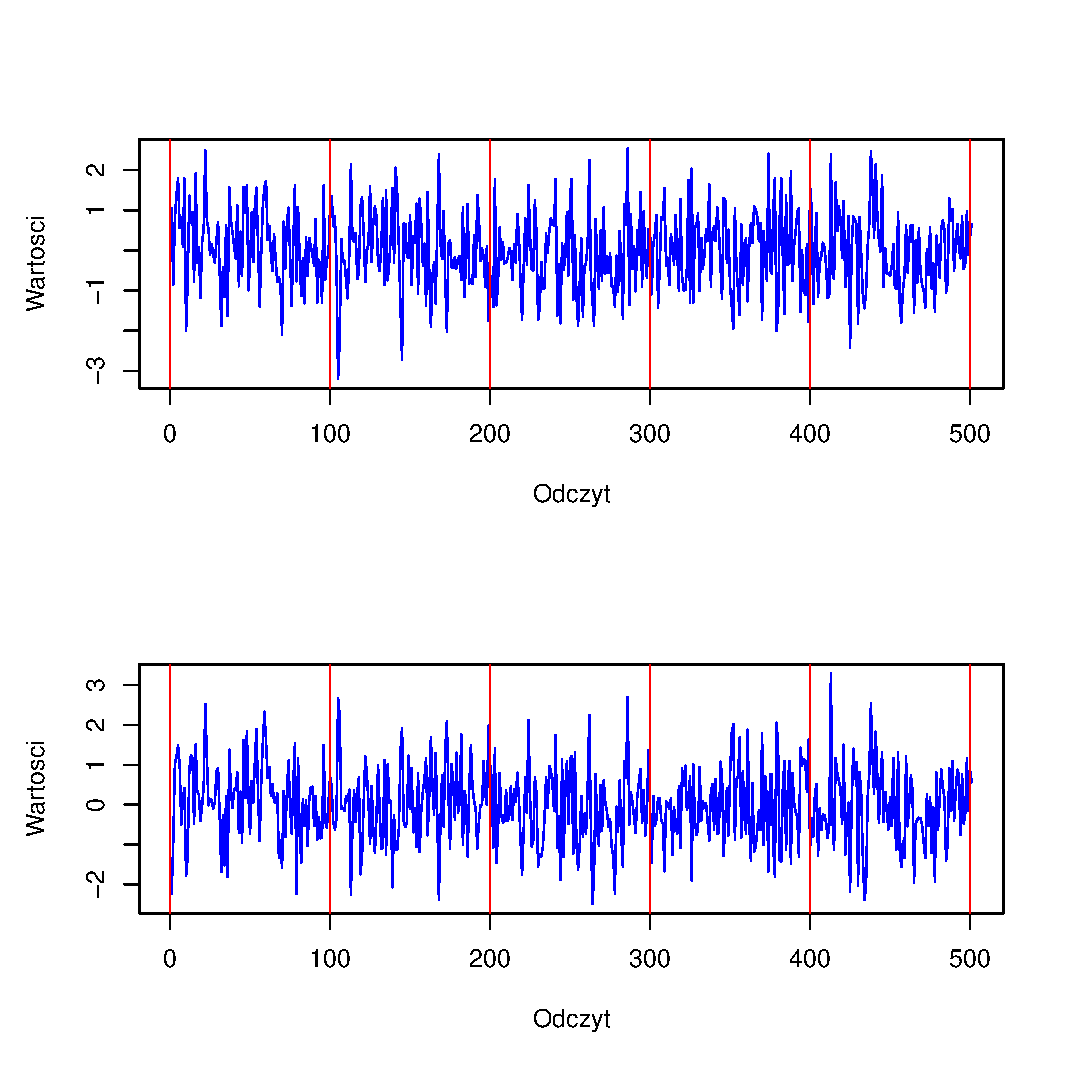
\includegraphics[width=0.8\textwidth]{img/ch-5-cov}
  \caption{Przykładowe wartości}
  \label{fig:CovValues}
\end{figure}
Na górnym rysunku przedstawiono pierwszy wymiar, na niższym drugi.
Badanie przeprowadzono poprzez wygenerowanie 20 zestawów danych.
